

\tikzset{every picture/.style={line width=0.75pt}} %set default line width to 0.75pt        

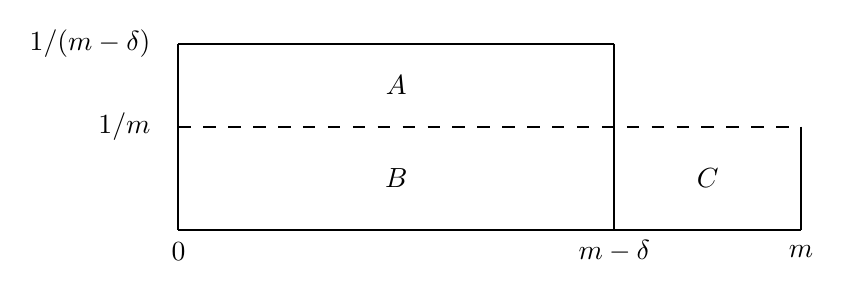
\begin{tikzpicture}[x=0.75pt,y=0.75pt,yscale=-1,xscale=1]
%uncomment if require: \path (0,300); %set diagram left start at 0, and has height of 300

%Straight Lines [id:da44485393234819215] 
\draw    (70,140) -- (370,140) ;
%Straight Lines [id:da865188063783277] 
\draw    (70,50) -- (70,140) ;
%Straight Lines [id:da19158122915410059] 
\draw    (70,50) -- (280,50) ;
%Straight Lines [id:da38010593816585625] 
\draw    (280,50) -- (280,140) ;
%Straight Lines [id:da8880042968224386] 
\draw  [dash pattern={on 4.5pt off 4.5pt}]  (70,90) -- (370,90) ;
%Straight Lines [id:da40410564631236867] 
\draw    (370,90) -- (370,140) ;

% Text Node
\draw (175,70) node    {$A$};
% Text Node
\draw (175,115) node    {$B$};
% Text Node
\draw (325,115) node    {$C$};
% Text Node
\draw (70,150) node    {$0$};
% Text Node
\draw (280,150) node    {$m-\delta $};
% Text Node
\draw (370,150) node    {$m$};
% Text Node
\draw (58,90) node [anchor=east] [inner sep=0.75pt]    {$1/m$};
% Text Node
\draw (58,50) node [anchor=east] [inner sep=0.75pt]    {$1/( m-\delta )$};


\end{tikzpicture}